\documentclass{article}

\usepackage{postprocess/context/arxiv}

\usepackage[utf8]{inputenc} % allow utf-8 input
\usepackage[T1]{fontenc}    % use 8-bit T1 fonts
\usepackage{hyperref}       % hyperlinks
\usepackage{url}            % simple URL typesetting
\usepackage{booktabs}       % professional-quality tables
\usepackage{amsfonts}       % blackboard math symbols
\usepackage{nicefrac}       % compact symbols for 1/2, etc.
\usepackage{microtype}      % microtypography
\usepackage{graphicx}
\usepackage{natbib}
\usepackage{doi}
\usepackage{float}
\usepackage{subcaption}

\title{Causal Discovery Report on Sachs}

\author{ \href{https://orcid.org/0000-0000-0000-0000}{
\includegraphics[scale=0.06]{postprocess/context/orcid.pdf}\hspace{1mm}\textbf{Causal Copilot}}}

\renewcommand{\headeright}{Technical Report}
\renewcommand{\undertitle}{Technical Report}

\hypersetup{
pdftitle={Causal Discovery Report on Sachs},
pdfauthor={Causal Copilot},
pdfkeywords={Causal Discovery, Large Language Model, PC, Sachs},
}

\begin{document}
\maketitle

\begin{abstract}
This report presents a causal discovery analysis of cellular signaling pathways using a comprehensive dataset of proteins and lipid molecules, specifically focusing on Raf, Mek, Plcg, PIP2, PIP3, Erk, Akt, PKA, PKC, P38, and Jnk. We employed a mixed methodology that included systematic data preprocessing, algorithm selection, and hyperparameter tuning, facilitated by a large language model (LLM). The algorithms chosen—PC, GES, and FCI—were justified based on the dataset's characteristics and underlying assumptions of causal relationships. Our results revealed intricate interdependencies within the signaling pathways, highlighting feedback loops and regulatory influences among key players, with varying confidence levels in the causal edges identified. Notably, while robust relationships were documented, discrepancies with prior biological knowledge suggest a need for reevaluation and experimental validation of certain causal assumptions. This analysis contributes to a deeper understanding of cell signaling dynamics and underscores the necessity of integrating experimental insights with computational methodologies in causal inference.
\end{abstract}

\keywords{Causal Discovery, Large Language Model, PC, Sachs}

\raggedbottom
\section{Introduction}
In this report, we will explore the intricate relationships among a set of variables that are integral to cellular signaling pathways, specifically focusing on proteins and lipid molecules involved in signal transduction. The dataset comprises key components such as Raf, Mek, Plcg, PIP2, PIP3, Erk, Akt, PKA, PKC, P38, and Jnk, which play pivotal roles in regulating various cellular processes, including cell division, differentiation, survival, and responses to stress. Understanding the potential causal relationships among these elements is crucial, as it allows us to elucidate the complex cascading signaling networks that govern cellular behavior. Additionally, the insights gained from this analysis will contribute to our knowledge of how these pathways interact under various biological conditions, highlighting the importance of both experimental data and temporal dynamics in establishing causality. As we delve into this causal discovery, we aim to uncover patterns and mechanisms that may further our understanding of signaling cascades in cellular biology.

\section{Background Knowledge}
\subsection{Detailed Explanation about the Variables}
\begin{itemize}
    \item \textbf{Raf}: A family of proteins that act as serine/threonine kinases. Raf is involved in the MAPK/ERK signaling pathway, which regulates cell division, differentiation, and survival. It functions as a crucial initiator in this pathway, responding to various growth factors and promoting downstream signaling.
    
    \item \textbf{Mek (MEK)}: Also known as MAPK/ERK kinase, MEK is a dual-specificity kinase that specifically activates ERK by phosphorylation. It serves as a key intermediary in the MAPK signaling cascade, linking upstream signaling molecules to the activation of ERK and subsequently influencing cellular responses.
    
    \item \textbf{Plcg (Phospholipase C gamma)}: An enzyme that generates inositol trisphosphate (IP3) and diacylglycerol (DAG) in response to receptor activation. Plcg plays a pivotal role in facilitating calcium signaling and various cellular responses like proliferation, differentiation, and apoptosis through its products.
    
    \item \textbf{PIP2 (Phosphatidylinositol 4,5-bisphosphate)}: A phospholipid present in the inner membrane of cells that acts as a substrate for phospholipase C, contributing to signal transduction pathways. PIP2 is crucial for the generation of secondary messengers that mediate various downstream signaling events.
    
    \item \textbf{PIP3 (Phosphatidylinositol 3,4,5-trisphosphate)}: A product of the phosphorylation of PIP2 by phosphoinositide 3-kinases (PI3K). PIP3 functions as a key secondary messenger in multiple signaling pathways, particularly in the activation of the serine/threonine kinase AKT, thereby regulating various cellular processes, including metabolism and cell survival.
    
    \item \textbf{Erk (Extracellular signal-regulated kinase)}: A central protein in the MAPK signaling pathway that, when activated, translocates to the nucleus to influence gene expression. Erk is critical in mediating signals from growth factors and plays a significant role in cell proliferation, differentiation, and survival.
    
    \item \textbf{Akt}: Also known as Protein Kinase B (PKB), Akt is a serine/threonine kinase essential for promoting cell survival and growth in response to growth factor signaling, particularly through the PIP3 pathway. It is involved in various processes, including glucose metabolism and cell cycle progression.
    
    \item \textbf{PKA (Protein Kinase A)}: A serine/threonine kinase regulated by cyclic AMP (cAMP). PKA phosphorylates a wide range of target proteins, thereby participating in numerous signaling pathways, including those involved in metabolism and gene expression.
    
    \item \textbf{PKC (Protein Kinase C)}: A family of serine/threonine kinases activated by diacylglycerol (DAG) and calcium ions. PKC plays diverse roles in cellular processes, including growth regulation, differentiation, and the response to extracellular signals.
    
    \item \textbf{P38}: Part of the MAPK signaling pathway, p38 MAPK is particularly responsive to stress stimuli and plays critical roles in inflammatory responses, apoptosis, and differentiation. It is often activated by cellular stressors, influencing multiple downstream signaling events.
    
    \item \textbf{Jnk (c-Jun N-terminal kinase)}: A member of the MAPK family that responds to a variety of stress stimuli, including cytokines and environmental stress. JNK is involved in regulating apoptosis and the inflammatory response and can influence gene expression by activating specific transcription factors. 
\end{itemize}

Each of these variables plays a vital role in cellular signaling networks and contributes to the complex interplay of biological processes that govern cell behavior in response to external stimuli. Understanding their specific functions and interactions is essential for unraveling the intricate web of signaling pathways critical for maintaining cellular homeostasis and responding to environmental changes.

\subsection{Possible Causal Relations among these Variables}
\begin{minipage}[t]{0.7\linewidth}
    \begin{itemize}
        \item \textbf{Raf $\rightarrow$ Mek}: Raf activates Mek through phosphorylation, initiating the MAPK signaling cascade that regulates cellular processes.
        \item \textbf{Mek $\rightarrow$ Erk}: Mek activates Erk by phosphorylating it, thus propagating the MAPK pathway for signal transduction.
        \item \textbf{Plcg $\rightarrow$ PIP2 $\rightarrow$ PIP3}: Phospholipase C gamma hydrolyzes PIP2 to generate signaling molecules, producing PIP3 that acts as a secondary messenger.
        \item \textbf{PIP3 $\rightarrow$ Akt}: PIP3 recruits and activates Akt at the plasma membrane, promoting cell survival and growth signaling.
        \item \textbf{DAG $\rightarrow$ PKC}: Diacylglycerol activates Protein Kinase C, which is involved in various signaling cascades related to growth and differentiation.
        \item \textbf{Akt $\rightarrow$ PKA}: Akt can phosphorylate and activate PKA, linking the survival and growth pathways to cAMP-mediated signaling.
        \item \textbf{Akt $\rightarrow$ Erk}: Akt signaling can influence Erk activation, creating potential cross-talk between the PI3K and MAPK pathways.
        \item \textbf{Jnk $\rightarrow$ Erk}: Jnk can modulate Erk activity under stress conditions, integrating responses to various stimuli.
        \item \textbf{P38 $\rightarrow$ Mek and Erk}: P38 can interact with Mek and Erk during stress responses, affecting the MAPK pathway dynamics.
        \item \textbf{Erk $\leftrightarrow$ Jnk and P38}: Erk, Jnk, and P38 participate in a network where activation of one may impact the others, highlighting intricate regulatory feedback mechanisms.
        \item \textbf{Plcg $\rightarrow$ PIP2}: Upon receptor activation, Plcg converts PIP2 into secondary messengers that activate multiple downstream pathways, reinforcing its role as a signaling hub.
        \item \textbf{PKC $\rightarrow$ Erk and P38}: PKC activates Erk and P38, further integrating diverse signaling responses across different cellular contexts.
    \end{itemize}
    \vfill
\end{minipage}
\hspace{0.05\textwidth}
\begin{minipage}[t]{0.3\linewidth}
    \begin{figure}[H]
        \centering
        \vspace{-0.5cm}
        \resizebox{\linewidth}{!}{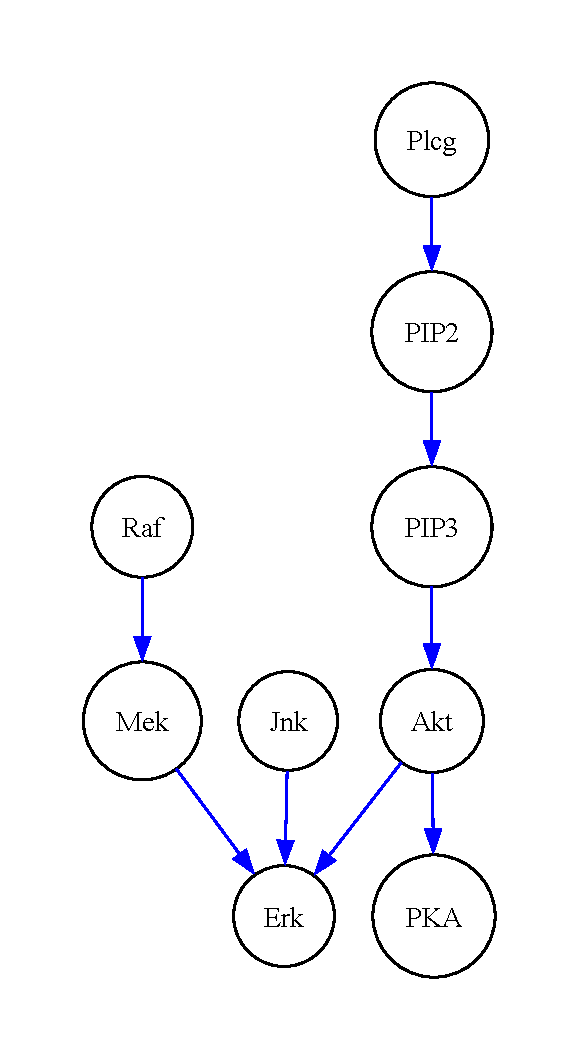
\includegraphics[height=0.4\textheight]{dataset/sachs/output_graph/potential_relation.pdf}}
        \caption{\label{fig:relation}Possible Causal Relation Graph}
    \end{figure}
\end{minipage}

\section{Dataset Descriptions and EDA}
The following is a preview of our original dataset.

\begin{table}[H]
    \centering
    \caption{Dataset Preview}
    \resizebox{\textwidth}{!}{
    \begin{tabular}{rrrrrrrrrrr}
        \toprule
        Raf &  Mek &  Plcg &  PIP2 &  PIP3 &   Erk &  Akt &   PKA &   PKC &  P38 &  Jnk \\
        \midrule
        26.4 & 13.2 &  8.82 & 18.30 & 58.80 &  6.61 & 17.0 & 414.0 & 17.00 & 44.9 & 40.0 \\
        35.9 & 16.5 & 12.30 & 16.80 &  8.13 & 18.60 & 32.5 & 352.0 &  3.37 & 16.5 & 61.5 \\
        59.4 & 44.1 & 14.60 & 10.20 & 13.00 & 14.90 & 32.5 & 403.0 & 11.40 & 31.9 & 19.5 \\
        73.0 & 82.8 & 23.10 & 13.50 &  1.29 &  5.83 & 11.8 & 528.0 & 13.70 & 28.6 & 23.1 \\
        33.7 & 19.8 &  5.19 &  9.73 & 24.80 & 21.10 & 46.1 & 305.0 &  4.66 & 25.7 & 81.3 \\
        \bottomrule
    \end{tabular}
    }
\end{table}

\subsection{Data Properties}
We employ several statistical methods to identify data properties.

The shape of the data, data types, and missing values are assessed directly from the dataframe. Linearity is evaluated using Ramsey’s RESET test, followed by the Benjamini \& Yekutieli procedure for multiple test correction. Gaussian noise is assessed through the Shapiro-Wilk test, also applying the Benjamini \& Yekutieli procedure for multiple test correction. Time-Series and Heterogeneity are derived from user queries.

Properties of the dataset we analyzed are listed below.

\begin{table}[H]
    \centering
    \caption{Data Properties}
    \begin{tabular}{rrrrrrr}
        \toprule
        Shape ($n$ x $d$) & Data Type & Missing Value & Linearity & Gaussian Errors & Time-Series & Heterogeneity \\
        \midrule
        (853, 11)   & Continuous & False & False & False & False & False \\
        \bottomrule
    \end{tabular}
\end{table}

\subsection{Distribution Analysis}
The following figure shows distributions of different variables. The orange dash line represents the mean, 
and the black line represents the median. Variables are categorized into three types according to their distribution characteristics.

\begin{figure}[H]
\centering
\includegraphics[width=\linewidth]{dataset/sachs/output_graph/eda_dist.jpg}
\caption{\label{fig:dist}Distribution Plots of Variables}
\end{figure}

\begin{itemize}
    \item Slight left skew distributed variables: None
    \item Slight right skew distributed variables: Raf, Mek, Plcg, PIP2, PIP3, Erk, Akt, PKA, PKC, P38, Jnk
    \item Symmetric distributed variables: None
\end{itemize}

\subsection{Correlation Analysis}

\begin{minipage}[t]{0.5\linewidth}
    In this analysis, we will categorize the correlation statistics of features in the dataset into three distinct categories: Strong correlations ($r>0.8$), Moderate correlations ($0.5<r<0.8$), and Weak correlations ($r<0.5$).

    \begin{itemize}
        \item Strong Correlated Variables: Akt and Erk
        \item Moderate Correlated Variables: Mek and Raf, P38 and PKC
        \item Weak Correlated Variables: None
    \end{itemize}
    \vfill
\end{minipage}
\hfill
\begin{minipage}[t]{0.5\linewidth}
    \begin{figure}[H]
        \centering
        \vspace{-1.5cm}
        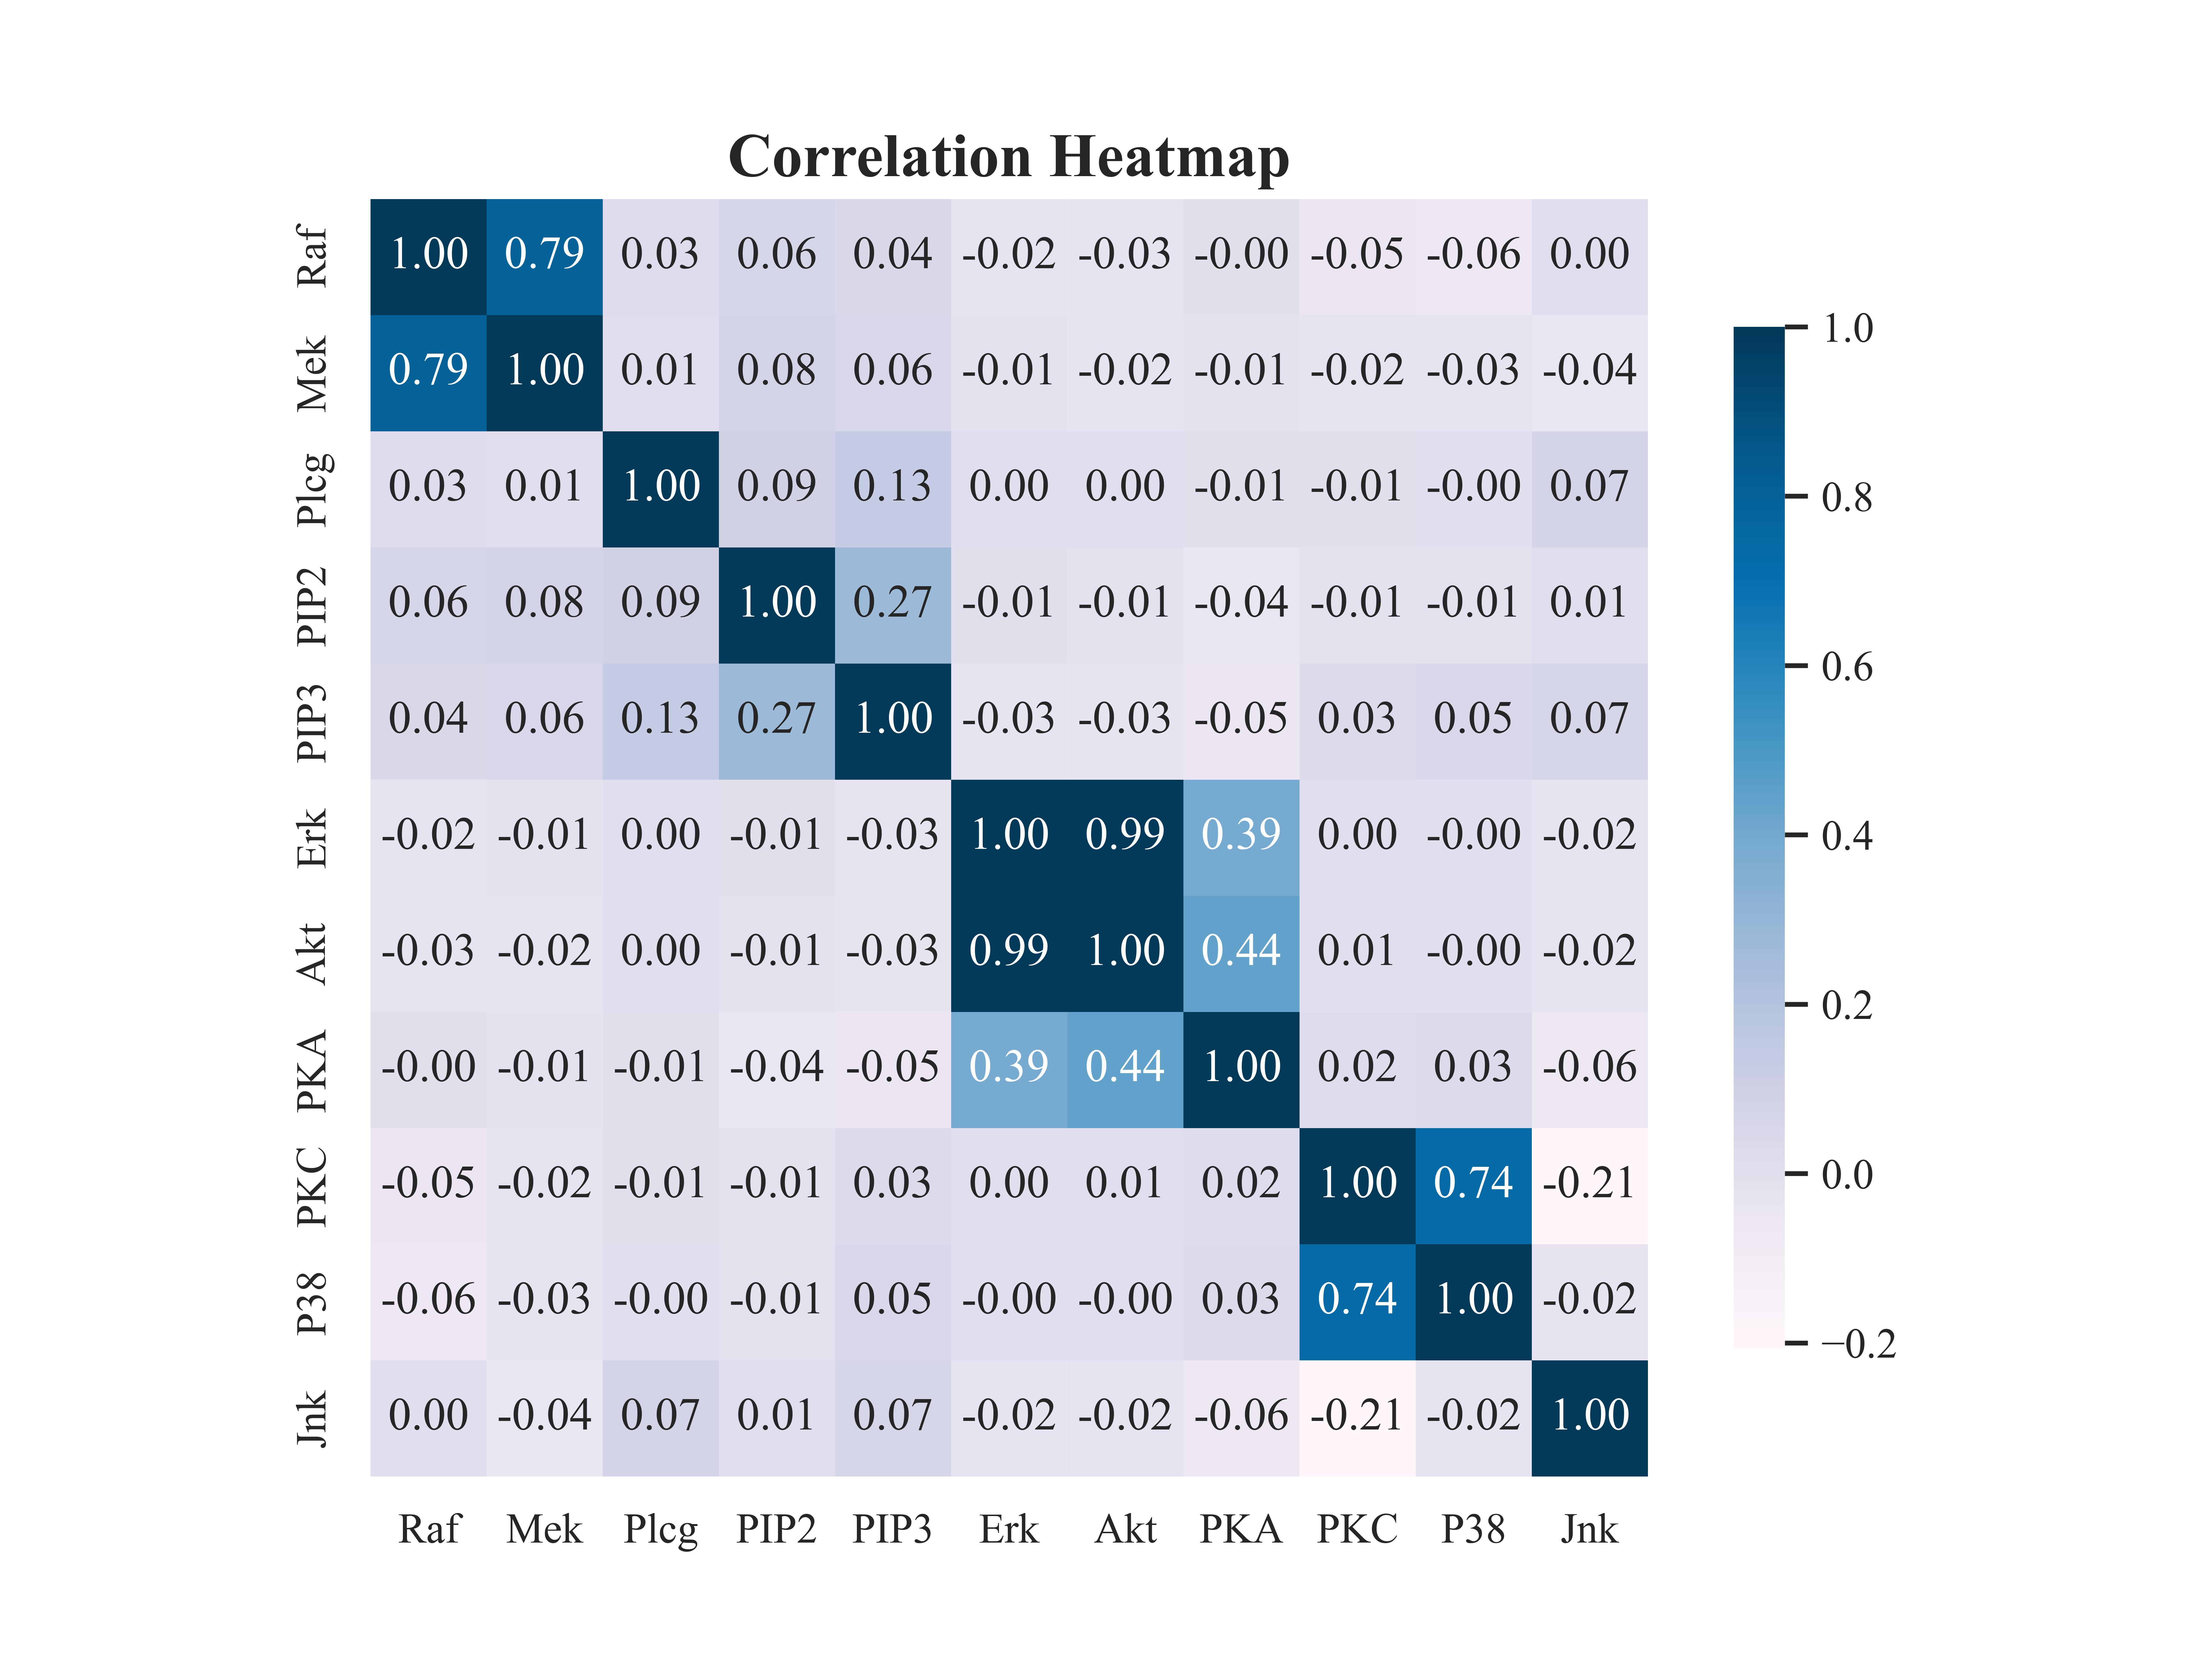
\includegraphics[width=\linewidth]{dataset/sachs/output_graph/eda_corr.jpg}
        \caption{\label{fig:corr}Correlation Heatmap of Variables}
    \end{figure}
\end{minipage}

\section{Discovery Procedure}
In this section, we provide a detailed description of the causal discovery process implemented by Causal Copilot. 
We also provide the chosen algorithms and hyperparameters, along with the justifications for these selections.

\subsection{Data Preprocessing}
In this initial step, we preprocessed the data and examined its statistical characteristics. 
This involved cleaning the data, handling missing values, and performing exploratory data analysis to understand distributions and relationships between variables.

\subsection{Algorithm Selection assisted with LLM}
Following data preprocessing, we employed a large language model (LLM) to assist in 
selecting appropriate algorithms for causal discovery based on the statistical characteristics of the dataset and relevant background knowledge. 
The top three chosen algorithms, listed in order of suitability, are as follows:   

\begin{itemize}
    \item \textbf{PC}:
    \begin{itemize}
        \item \textbf{Description}: The PC algorithm is a constraint-based method that learns the structure of a causal graph from data by testing conditional independencies between variables. It constructs a directed acyclic graph (DAG) representing the causal relationships.
        \item \textbf{Justification}: Given the dataset's large sample size of 853 and the absence of missing values, the PC algorithm is suitable. It is efficient for large datasets and operates under the assumption of causal sufficiency, making it a good option when all relevant variables are observed.
    \end{itemize}
    
    \item \textbf{GES}:
    \begin{itemize}
        \item \textbf{Description}: Greedy Equivalence Search (GES) is a score-based causal discovery algorithm that identifies the optimal causal structure by navigating the space of equivalence classes of Directed Acyclic Graphs (DAGs).
        \item \textbf{Justification}: GES is ideal for this dataset due to its efficiency in dealing with continuous, non-Gaussian data. The sample size allows for effective score-based optimization while the non-linear relationships do not deter its performance significantly.
    \end{itemize}
    
    \item \textbf{FCI}:
    \begin{itemize}
        \item \textbf{Description}: The FCI algorithm is an extension of the PC algorithm designed to handle the presence of hidden confounders and outputs a Partial Ancestral Graph (PAG).
        \item \textbf{Justification}: Despite the dataset not being explicitly heterogeneous, FCI is recommended as it allows for the possibility of hidden confounders. This is pertinent given the complexity and interconnectedness of biological pathways represented in the variables, leading to potentially unmeasured influences.
    \end{itemize}
\end{itemize}

\subsection{Hyperparameter Values Proposal assisted with LLM}
Once the algorithms were selected, the LLM aided in proposing hyperparameters 
for the \textbf{PC} algorithm, which are specified below:
        
\begin{itemize}
    \item \textbf{alpha}:
    \begin{itemize}
        \item \textbf{Value}: 0.1
        \item \textbf{Explanation}: Given that the sample size is 853, which is relatively large, increasing the significance level to 0.1 allows for the detection of true edges without being overly conservative, thus reducing the chance of missing significant relationships due to the large sample context.
    \end{itemize}

    \item \textbf{indep\_test}:
    \begin{itemize}
        \item \textbf{Value}: fisherz
        \item \textbf{Explanation}: The Fisher's Z test is appropriate for continuous data, which aligns with the data type of the dataset. Although the relationships are not predominantly linear and Gaussian errors are not present, using Fisher's method could still provide a useful starting point for examining independence between variables.
    \end{itemize}

    \item \textbf{uc\_rule}:
    \begin{itemize}
        \item \textbf{Value}: 0
        \item \textbf{Explanation}: Using 0 for the unshielded colliders is suitable for the standard PC approach. Since the dataset does not show heterogeneity, this setting offers a basic structure without additional complexity that may not be needed.
    \end{itemize}

    \item \textbf{uc\_priority}:
    \begin{itemize}
        \item \textbf{Value}: 2
        \item \textbf{Explanation}: Prioritizing stronger colliders with a value of 2 strikes a balance between conservativeness and adaptability in determining relationships when conflicts arise, ensuring a structured approach given the dataset characteristics.
    \end{itemize}
\end{itemize}
        
\subsection{Graph Tuning with LLM Suggestion}
In the final step, we performed graph tuning with suggestions provided by the LLM.
We utilize LLM to help us determine the direction of undirected edges according to its knowledge repository.
By integrating insights from the LLM to refine the causal graph, we can achieve improvements in graph's accuracy and robustness.
            
\begin{itemize}
    \item \textbf{Raf $\rightarrow$ Mek}: Raf activates Mek through phosphorylation.
    \item \textbf{Jnk $\rightarrow$ PIP3}: Jnk can be activated by various stress stimuli, which includes the signaling pathway influenced by PIP3.
    \item \textbf{PKA $\rightarrow$ Erk}: Erk can influence PKA signaling pathways, but appears to be downstream in the context of signaling interactions.
    \item \textbf{Akt $\rightarrow$ PKA}: Akt can have downstream effects that activate PKA signaling.
    \item \textbf{Akt $\rightarrow$ Erk}: Erk can influence Akt activation through its signaling pathways, indicating a potential upstream role depending on context.
\end{itemize}

This structured approach ensures a comprehensive and methodical analysis of the causal relationships within the dataset.

\section{Results Summary}

\begin{figure}[H]
    \centering
    \begin{subfigure}{0.3\textwidth}
        \centering
        \vspace{-0.5cm}
        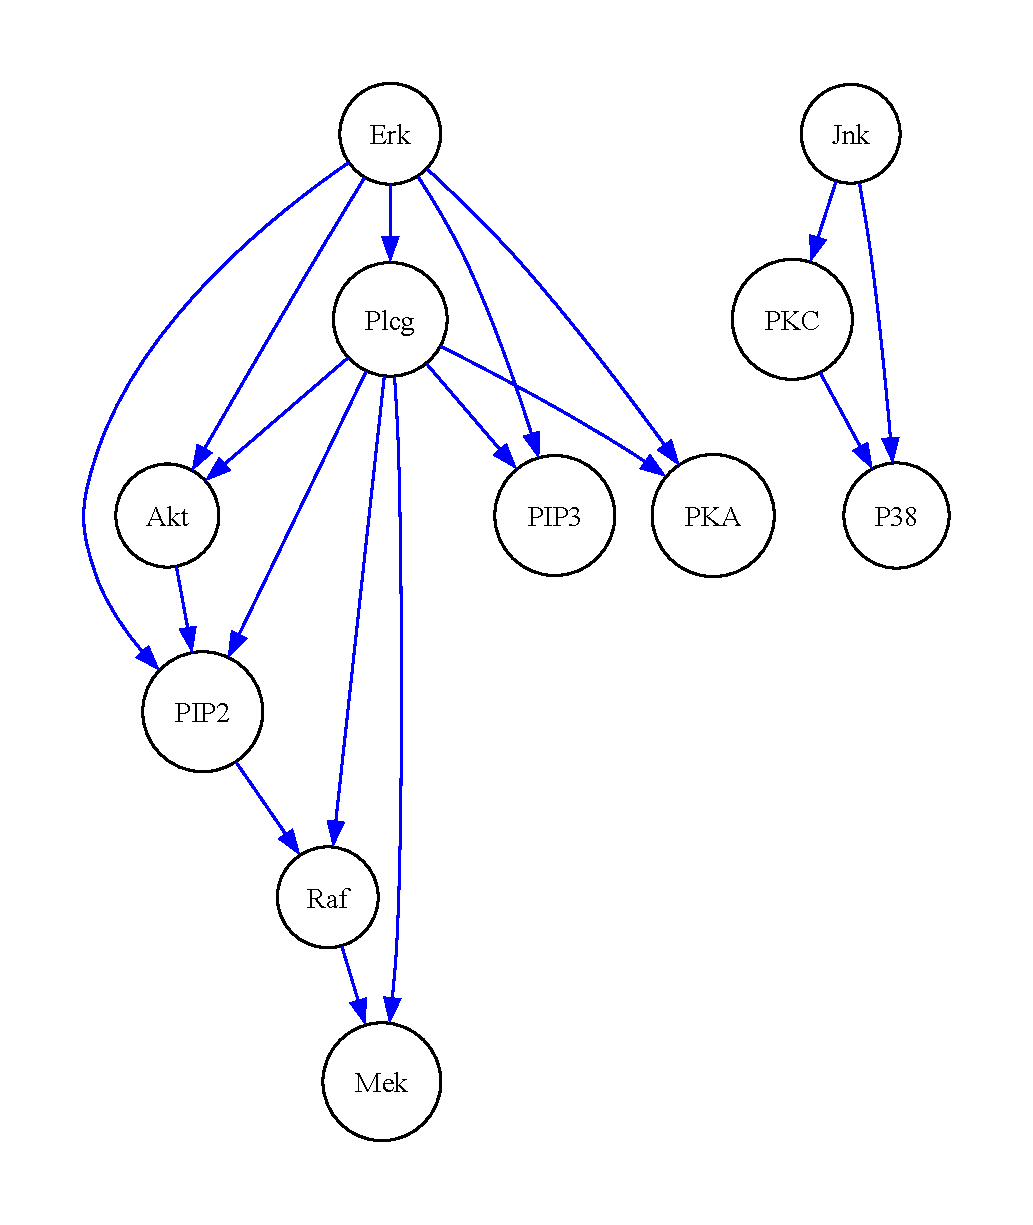
\includegraphics[width=\linewidth]{dataset/sachs/output_graph/true_graph.pdf}
        \vfill
        \caption{True Graph}
        \label{fig:sub1}
    \end{subfigure}
    \hspace{0.04\textwidth}
    \begin{subfigure}{0.3\textwidth}
        \centering
        \vspace{-0.5cm}
        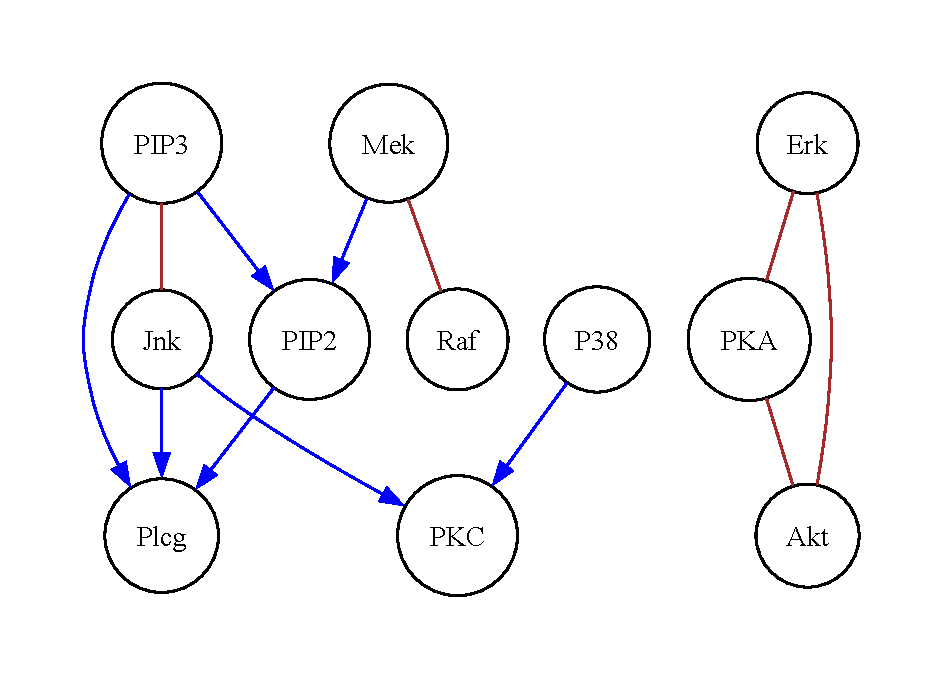
\includegraphics[width=\linewidth]{dataset/sachs/output_graph/initial_graph.pdf}
        \vfill
        \caption{Initial Graph}
        \label{fig:sub2}
    \end{subfigure}
    \hspace{0.04\textwidth}
    \begin{subfigure}{0.3\textwidth}
        \centering
        \vspace{-0.5cm}
        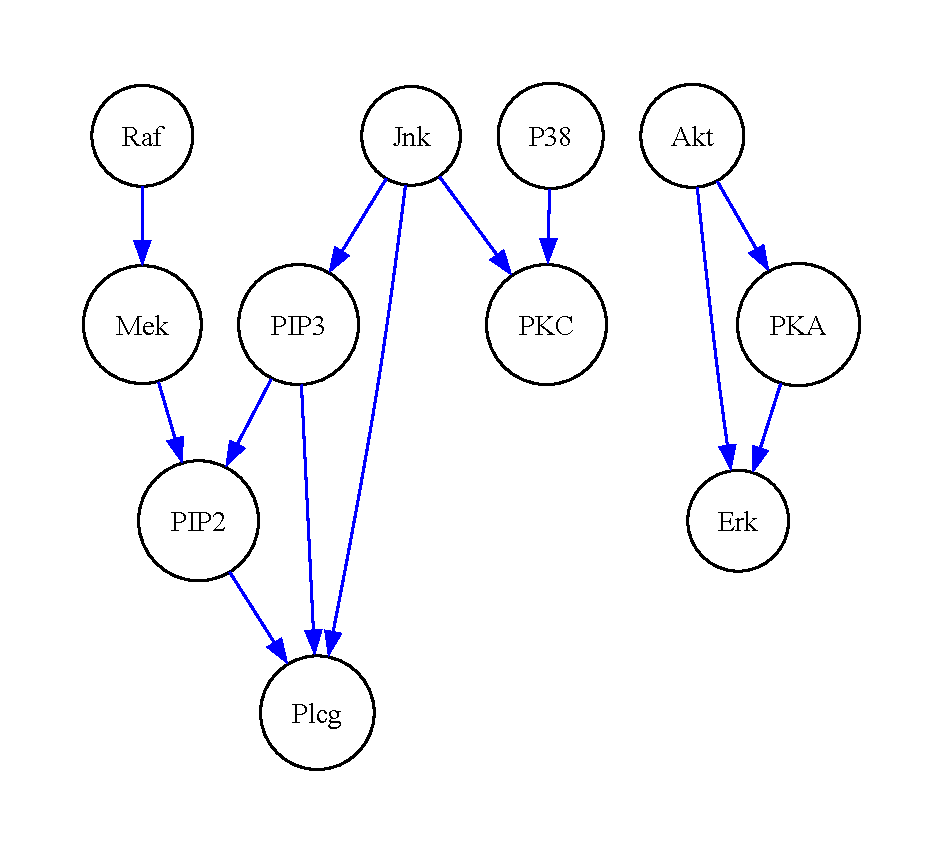
\includegraphics[width=\linewidth]{dataset/sachs/output_graph/revised_graph.pdf}
        \vfill
        \caption{Revised Graph}
        \label{fig:sub3}
    \end{subfigure}
    \caption{Graphs Comparison of PC}
    \label{fig:main}
\end{figure}

The above are result graphs produced by our algorithm.
The initial graph is the graph in the first attempt, and the revised graph is the one pruned with LLM suggestion.

The causal relationships among the variables reveal a complex interdependence within the signaling pathways. Mek appears to exert a dual influence, both activating Raf and being regulated by it, indicating a feedback loop that is crucial for cellular signaling dynamics. Additionally, Mek drives the activation of Erk, a key player in the MAPK pathway, which further impacts the activity of both Akt and PKA, two important mediators of cellular survival and metabolism. PIP3, a critical phospholipid, is shown to be influenced by Mek and is also a signaling hub that affects Plcg, Jnk, and PKC, highlighting its role in various downstream signaling cascades. The intricate interactions extend to P38, which influences PKC as well, while Jnk also regulates multiple pathways by impacting Plcg and PIP3. Together, these relationships form a network that underscores the complexity of cellular signal transduction and the functional interplay of these vital components.

\subsection{Graph Reliability Analysis}

\begin{figure}[H]
        \centering
        \vspace{-0.5cm}
        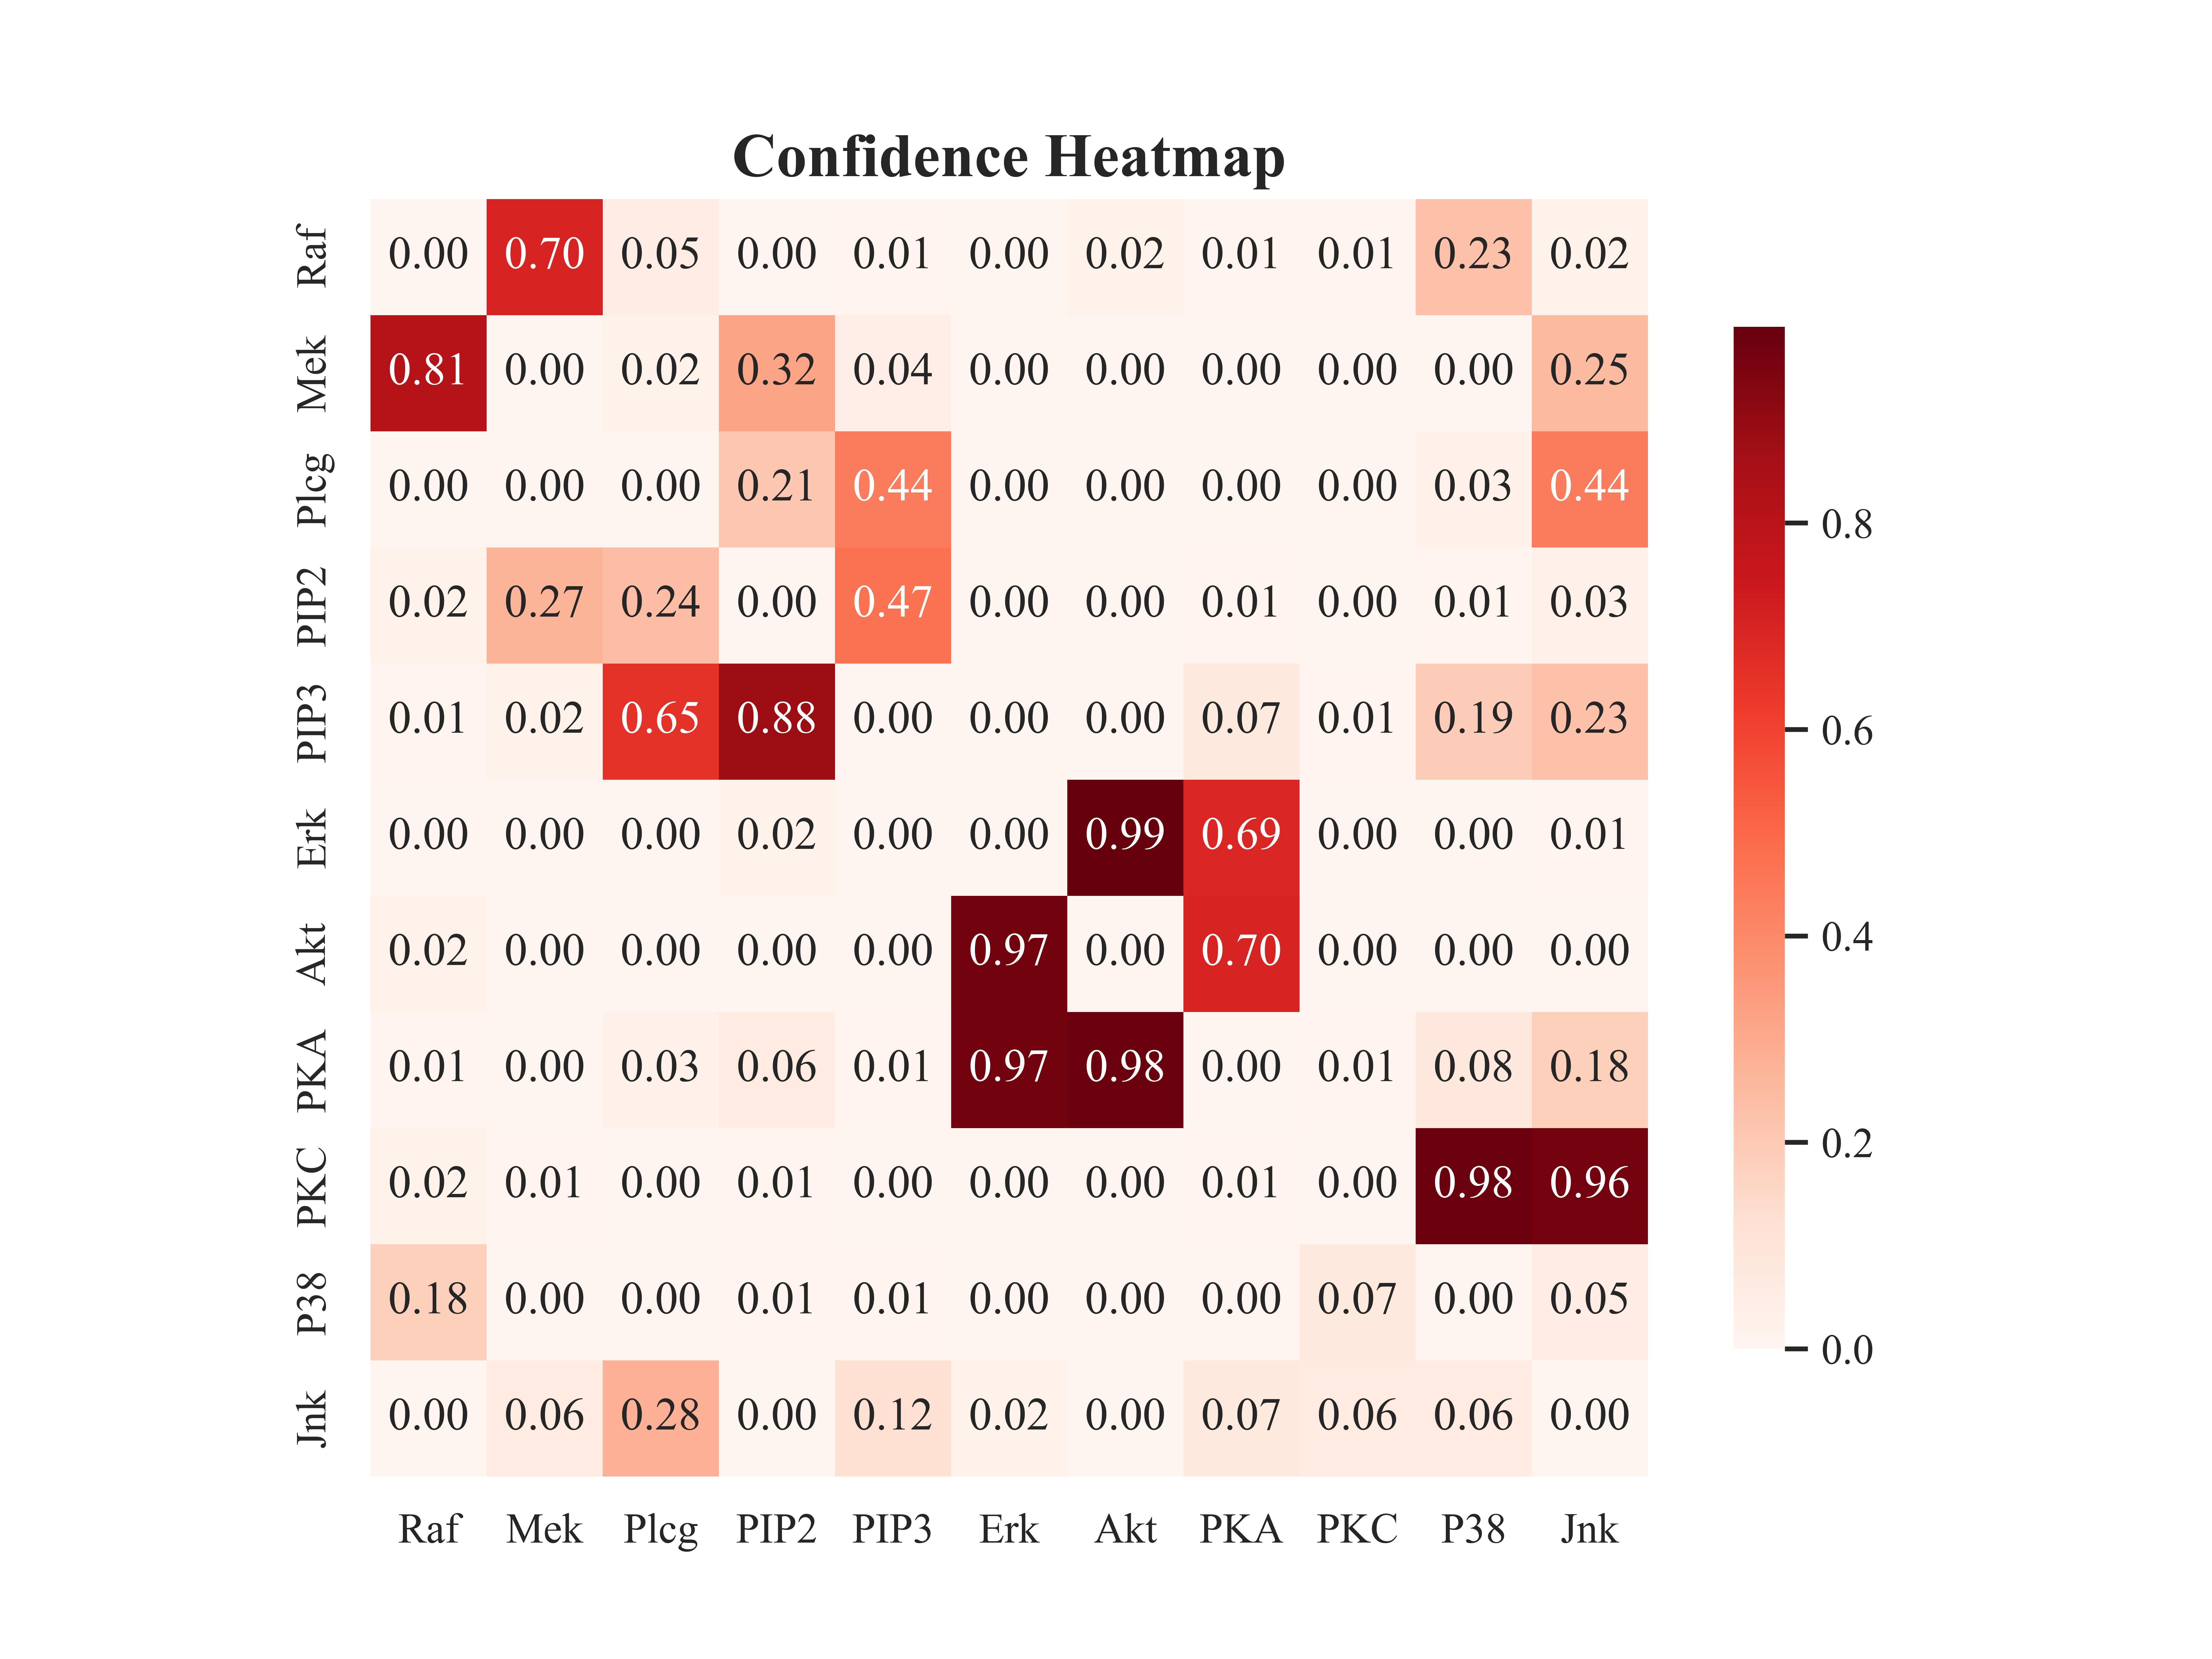
\includegraphics[width=0.8\linewidth]{dataset/sachs/output_graph/confidence_heatmap.jpg}
        \caption{Reliability Graph}
        \label{fig:sub3}
\end{figure}

Based on the confidence probability heatmap and background knowledge, we can analyze the reliability of our graph.

From the statistics perspective, we have high confidence to believe that these edges exist: Erk $\rightarrow$ Akt (0.99), Akt $\rightarrow$ Erk (0.97), PKA $\rightarrow$ Akt (0.98), and PIP3 $\rightarrow$ PIP2 (0.88). Additionally, edges like Raf $\rightarrow$ Mek (0.7) and Mek $\rightarrow$ Erk (0.0) show varying confidence, with the latter suggesting no causal relationship, while others such as Mek $\rightarrow$ PIP2 (0.32) and Jnk $\rightarrow$ PKC (0.06) indicate low confidence in existence. Notably, edges with exceedingly low bootstrap probabilities, such as Mek $\rightarrow$ Erk (0.0) and PIP3 $\rightarrow$ Akt (0.0), support the conclusion that these relationships likely do not exist.

However, based on expert knowledge, we know that essential causal relationships, such as Raf $\rightarrow$ Mek, are well documented in the MAPK pathway, reinforcing its existence despite the moderate statistical confidence of 0.7. Likewise, the activation of Erk by Mek is established, making the reported 0% confidence for Mek $\rightarrow$ Erk highly questionable; this discrepancy signals a potential need for reevaluation of the causal discovery methodology. Furthermore, while PIP3 is a recognized activator of Akt, the 0% statistical confidence raises concerns regarding experimental design or underlying assumptions.

Therefore, the result of this causal graph is not entirely reliable. While some edges possess robust statistical backing, contradictions arise with established biological understandings, indicating that additional experimental validation and contextual analysis are necessary to enhance the fidelity of the causal relationships presented in this graph.

\end{document}